% !TEX root = ../main.tex

\section{Introduction}



Ethereum is an open blockchain proposed in 2013 and deployed in 2015~\cite{Ref00}. At the time of writing, it has the second largest market value behind Bitcoin.\footnote{CoinMarketCap - Ethereum currency - Accessed: 2019-02-11 \newline\url{https://coinmarketcap.com/currencies/ethereum/}} It has a large development community which track enhancements and propose new ideas.\footnote{CoinDesk Crypto-Economics Explorer - Accessed: 2019-02-11 \newline\url{https://www.coindesk.com/data}} Ethereum enables decentralized applications (\dapps) to be deployed and run on it---DApps can accept and transfer Ethereum's built in currency (ETH). 

Commonly, DApps will issue their own custom currency-like tokens for specific purposes. Tokens might be currencies with different properties than ETH, they may be tokens that are required for access to a DApp's functionality, or they might represent ownership of some off-blockchain asset. It is beneficial to have tokens be interoperable with other DApps and off-blockchain webapps, such as exchange services that allow tokens with some market value to be traded. Toward this goal, the Ethereum project accepted a proposed standard (EIP20) for a set of methods that standard-compliant tokens (called ERC20 tokens) should implement. In terms of object oriented programming (most DApps are developed in a Java-like language called Solidty), ERC20 is an interface that defines abstract methods (name, parameters, return types) and provides guidance on how the methods should be implemented, but does not provide an actual concrete implementation. 


% the blockchain. Tokens are essential part of this ecosystem which define set of rules---known as API\footnote{Advanced Programming Interface.}---for standardizing interaction with smart contracts.\footnote{Types of transactions that execute as they are programmed by Ethereum scripting language (e.g., Solidity or Vyper)}. Therefore, any ERC20\footnote{ERC20 is title of the standard and it should be referred as EIP20 (which is the actual proposal for improvement). In this paper we use both ERC20 and EIP20 in one sense for simplicity.}-compliant application can interact with any ERC20 token for trading, swapping, exchanging, etc. For example, shares of company X can be represented as ERC20 tokens to be reusable by other smart contracts (e.g., online exchanges, automated payment systems, decentralized games, etc). Leveraging ERC20 token facilitates implementation of financial assets while raising some security concerns. ERC20 tokens are technically standardized version of smart contracts that could be similarly vulnerable to security flaws.

% Jeremy: This seems unnecessary:
%\begin{figure}[t]
%	\centering
%	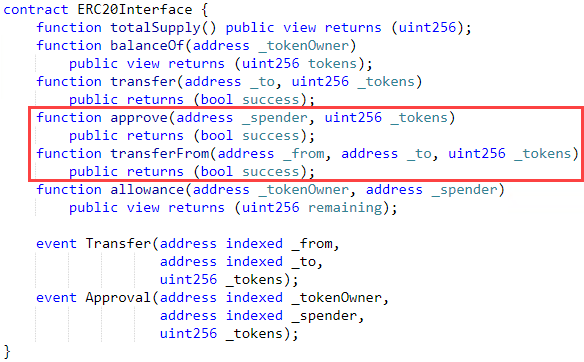
\includegraphics[width=1.0\linewidth]{figures/multiple_withdrawal_01.png}
%	\caption{Importance of ERC20 security in case of (1) digitizing share of company X (2) representing a fiat currency. In this case, smart contracts interact with two different ERC20 tokens which are repressing in sequence, a financial instrument and a non-collateralized stablecoin. Any security vulnerability in written code of ERC20 tokens, will impact security of related smart contracts and value of underlying assets.}
%\end{figure}

\begin{figure}[t!]
	\centering
	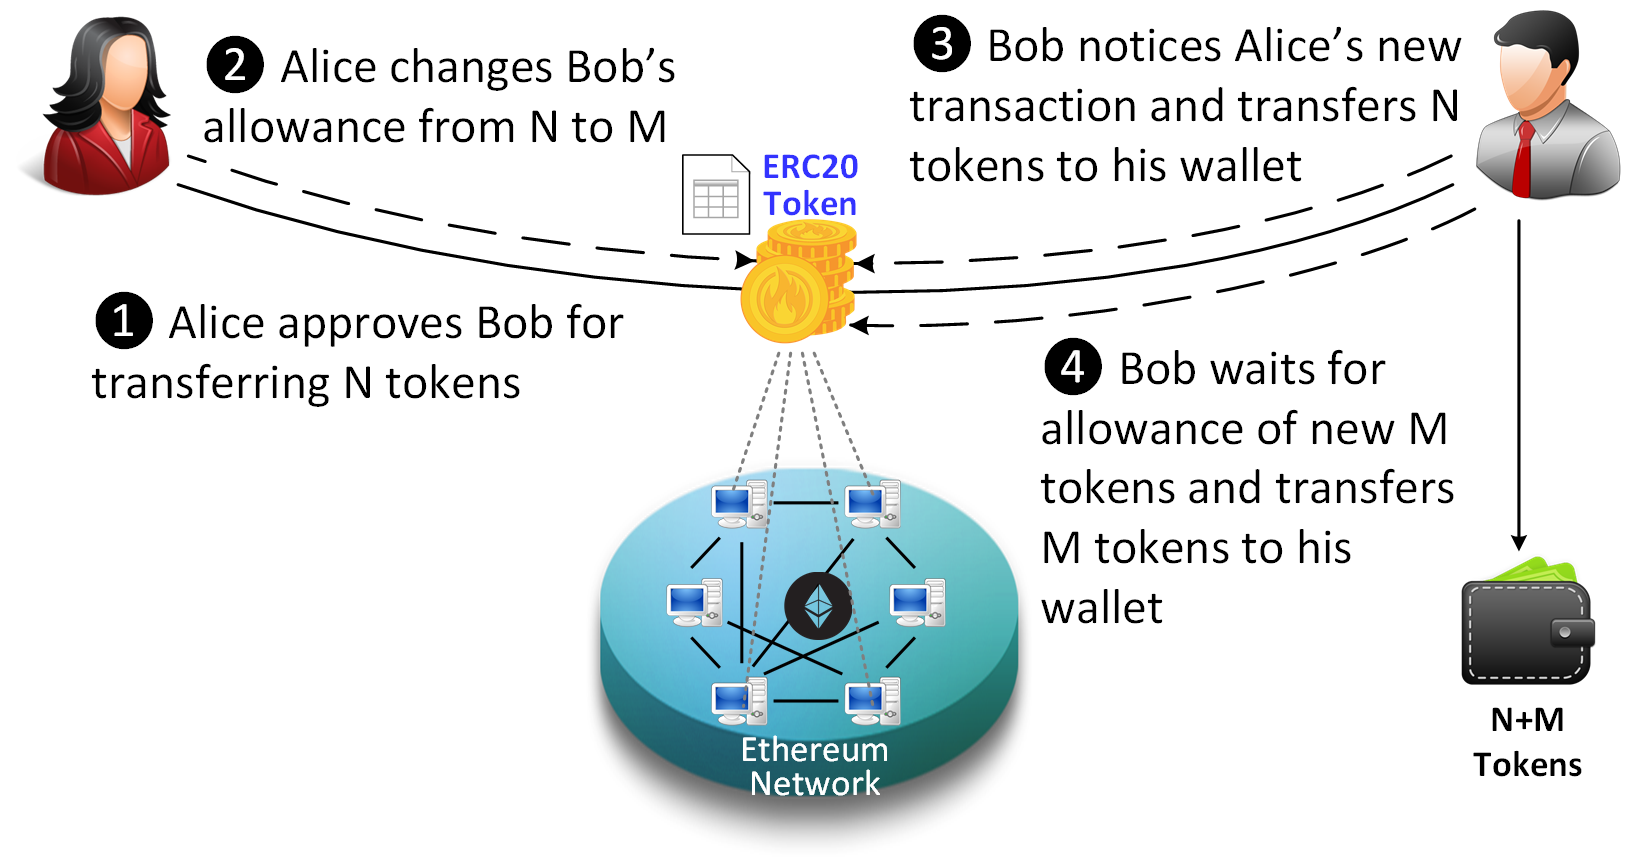
\includegraphics[width=1.0\linewidth]{figures/multiple_withdrawal_02.png}
	\caption{Possible multiple withdrawal attack in ERC20 tokens when Alice changes Bob's allowance from N to M. By front-running, Bob is able to move N+M tokens from Alice's token pool.\label{fig:mwa}}
\end{figure}

Since its introduction in November 2015, several vulnerabilities have been discovered in ERC20's design. In October 2017, the security issue called the ``Multiple Withdrawal Attack'' was opened on GitHub\cite{Ref13,Ref07}. The attack originates from how two methods in the ERC20 standard, methods for approving and transferring tokens, are described. The use of these functions in an undesirable situation (\eg front-running) could result in conditions that tokens being spent by another third party on behalf of the owner (see Figure~\ref{fig:mwa}). This issue is still open and several solutions have been made to mitigate it. We started off by analyzing two sample ERC20 tokens from OpenZeppelin\cite{Ref10} and ConsenSys\cite{Ref11} that advised as generic implementations by authors of ERC20 standard \cite{Ref08}. OpenZeppelin uses two additional methods and ConsenSys has not attempted to work around the issue. There are other implementations that have a variety of different trade-offs in solving this issue. 

\subsubsection*{Contributions} In this paper, we discuss 10 solutions to the multiple withdrawal attack and evaluate them according to a set of criteria we develop in terms of compatibility with the standard and attack mitigation (see the summary in Table~\ref{tab:comp}). Since none of them precisely satisfy the constraints of the ERC20 standard, we were motivated to propose new solutions to mitigate the attack. Specifically, we propose  two new approaches: each secures one of the two vulnerable methods (\ie \texttt{approve} or \texttt{transferFrom}). The first one, mitigates the attack by comparing transferred tokens with the current allowance in the \texttt{approve} method. The second proposal secures \texttt{transferFrom} method by not allowing token transfers more than allowed. Since the attack happens in the event of gap between transactions, we used compare and set (CAS) pattern\cite{Ref06} to cover this gap. CAS is one of the most widely used lock-free synchronization strategy that allows comparing and setting values in an atomic way. It allows to compare values in one transaction and set new values before transferring control to another one. We leveraged this pattern to remove the gap between transactions and prevent race condition as root cause of the attack. As shown in the Table~\ref{tab:comp}, Proposal 1 mitigates the attack but it is partially-ERC20-compliant. This is because of violation of one of ERC20 constraints that prohibits any adjustment in allowance. As we discuss, it would not be feasible to secure \texttt{approve} method without adjusting allowance. Alternatively, securing \texttt{transferFrom} method in Proposal 2 mitigate the attack effectively.

\begin{figure}[t!]
	\centering
	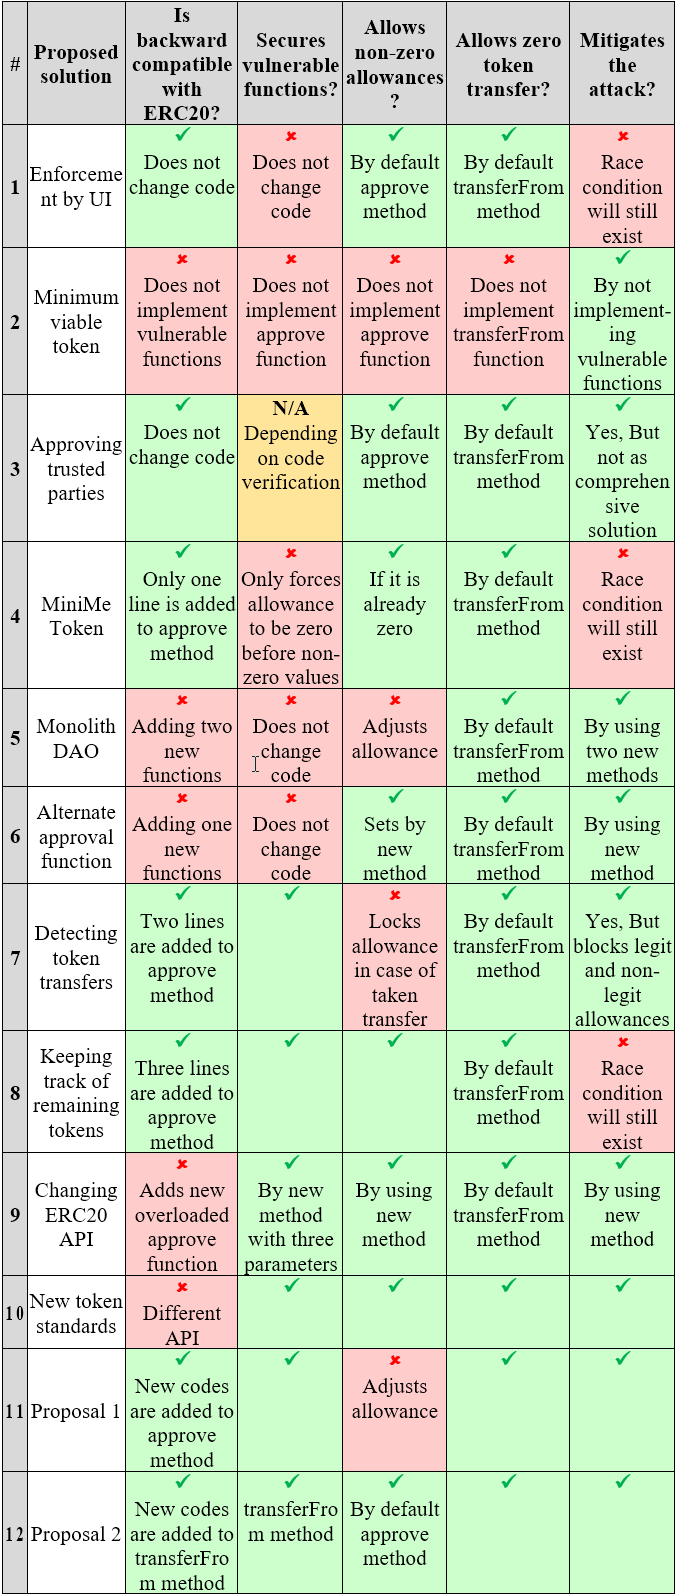
\includegraphics[width=1.0\linewidth]{figures/multiple_withdrawal_04.png}
	\caption{Comparison of 10 suggested solutions with two proposals contributed by this paper. Proposal 2 uses CAS pattern to mitigate the attack sustainably by (1) comparing transferred tokens through a new local variable in \texttt{transferFrom} function and (2) tracking of transferred tokens to prevent more transfers.\label{tab:comp}}
\end{figure}
